\section{Predição Linear}

\begin{frame}%[allowframebreaks]
  \frametitle{Predição Linear}
  Predição linear é uma operação matemática em que se utiliza valores passados de um sinal discreto no tempo para
  prever valores futuros deste mesmo sinal. Em processamento digital de sinais, a predição linear é conhecida como
  \emph{linear predictive coding (LPC)} e pode ser entendida no contexto de filtros digitais.
\end{frame}


\begin{frame}%[allowframebreaks]
  \frametitle{Aplicações da Predição Linear}
  \begin{itemize}
  \item Análise de sinais da fala;
  \item Análise de eletroencefalograma;
  \item Análise de sinais sísmicos;
  \item Estimação de Formantes da fala;
  \item Controle de Ruído;
  \item Controle;
  \item etc.
  \end{itemize}
\end{frame}


\subsection{Formulação Matemática}
\begin{frame}%[allowframebreaks]
  \frametitle{Formulação Matemática}
  O preditor linear de ordem $p$ é descrito pela equação:
  \begin{equation}
  \hat{x}(n) = \sum_{i=1}^{p} a_i x(n-i) .
  \end{equation}
 
  O erro de predição é dado por
  \begin{equation}
  e(n) = x(n) - \hat{x}(n) .
  \end{equation}

  O preditor é determinado pelos coeficientes $a_1, \ldots, a_p$.
\end{frame}


\begin{frame}%[allowframebreaks]
  \frametitle{Determinação do Preditor}
  Dado um sinal $x$ queremos encontrar o melhor preditor para este sinal.

  Melhor: erro de estimação mínimo (erro médio quadrático)

  Objetivo: minimizar o valor esperado do erro médio quadrático, $E\left[ \vert e(n) \vert^2 \right]$.
\end{frame} 


\begin{frame}%[allowframebreaks]
  \frametitle{Minimização do Valor Esperado do Erro Médio Quadrático}
  Para encontrar os parâmetros que minimizam o erro devemos buscar o conjunto de parâmetros que satisfaz:
  \begin{enumerate}
  \item derivada primeira nula em relação a cada um dos parâmetros $a_k$, $k=1,\ldots,p$
  \begin{equation}
  \frac{\partial E\left[ \vert e(n) \vert^2 \right]}{\partial a_k} = 0
  \end{equation}
  \item derivada segunda positiva em relação a cada um dos parâmetros $a_k$, $k=1,\ldots,p$
  \begin{equation}
  \frac{\partial^2 E\left[ \vert e(n) \vert^2 \right]}{\partial a_k^2} > 0
  \end{equation}
  \end{enumerate}
  Garantia de que encontraremos um mínimo qualquer, não necessariamente o mínimo global.
\end{frame} 


\begin{frame}%[allowframebreaks]
  \frametitle{Módulo Quadrado do Erro}
  \begin{eqnarray}
  \vert e(n) \vert^2 &=& e(n) e^\ast(n) \nonumber \\
        &=& (x(n) - \hat{x}(n)) e^\ast(n) \nonumber \\
        &=& \left( x(n) - \sum_{i=1}^p a_i x(n-i) \right) e^\ast(n) \nonumber \\
        &=& \left( x(n) e^\ast(n) \right) - \left( \sum_{i=1}^p a_i x(n-i) e^\ast(n) \right) 
  \end{eqnarray}
  logo
  \begin{equation}
  E\left[ \vert e(n) \vert^2 \right] = E\left[ x(n) e^\ast(n) \right] - \sum_{i=1}^p a_i E\left[ x(n-i) e^\ast(n) \right]
  \end{equation}
\end{frame} 


\begin{frame}%[allowframebreaks]
  \frametitle{Derivada}
  \begin{equation}
  E\left[ \vert e(n) \vert^2 \right] = E\left[ x(n) e^\ast(n) \right] - \sum_{i=1}^p a_i E\left[ x(n-i) e^\ast(n) \right] \nonumber
  \end{equation}

  \begin{eqnarray}
  \frac{\partial E\left[ \vert e(n) \vert^2 \right]}{\partial a_k} &=& 0 - E\left[ x(n-k) e^\ast(n) \right] \nonumber \\
       &=& - E\left[ x(n-k) \left( x(n) - \hat{x}(n) \right)^\ast \right] \nonumber \\
       &=& - E\left[ x(n-k) \left( x(n) - \sum_{i=1}^p a_i x(n-i) \right)^\ast \right] \nonumber \\
       &=& - E\left[ x(n-k) \left( x^\ast(n) - \sum_{i=1}^p a_i^\ast x^\ast(n-i) \right) \right] \nonumber
  \end{eqnarray}
\end{frame} 


\begin{frame}%[allowframebreaks]
  \frametitle{Derivada}
  Queremos
  \begin{eqnarray}
  \frac{\partial E\left[ \vert e(n) \vert^2 \right]}{\partial a_k} &=& 0  \\
  - E\left[ x(n-k) x^\ast(n) \right] + && \nonumber \\
   \sum_{i=1}^p a_i^\ast E\left[ x^\ast(n-i) x(n-k) \right] &=& 0 \nonumber \\
  \sum_{i=1}^p a_i^\ast E\left[ x^\ast(n-i) x(n-k) \right]  &=& E\left[ x(n-k) x^\ast(n) \right] \nonumber \\
  \sum_{i=1}^p a_i^\ast r(k-i) = r(k) \nonumber
  \end{eqnarray}
  aonde $r(k)$ é a autocorrelação do sinal $x(n)$ avaliada com deslocamento $k$.
\end{frame} 


\begin{frame}
  \frametitle{Autocorrelação}
  A autocorrelação do sinal $x(n)$ avaliada com deslocamento $k$ é dada por
  \begin{equation}
  r(k) = \lim_{N \rightarrow \infty} \frac{1}{N} \sum_{n=-N/2}^{N/2} x(n) x^\ast(n-k)
  \end{equation}

  A autocorrelação de sequências reais é simétrica e par. Desta forma, sendo $x(n)$ um sinal real,
  teremos $r(k) = r(-k)$.
\end{frame}

\begin{frame}
  \frametitle{Sistemas de Equações}
  Dado que
  \begin{equation}
  r(k) = \sum_{i=1}^p a_i^\ast r(k-i) ,
  \end{equation}
  vamos criar um sistema com $p$ equações tomando o deslocamento nulo ($k=0$) como referência.
  \begin{equation}
  \begin{cases} 
  r(1) = a_1 r(0) + a_2 r(1) + a_3 r(2) + \ldots + a_p r(p-1) \\
  r(2) = a_1 r(1) + a_2 r(0) + a_3 r(1) + \ldots + a_p r(p-2) \\
  \vdots \\
  r(p) = a_1 r(p-1) + a_2 r(p-2) + a_3 r(p-3) + \ldots + a_p r(0)  
  \end{cases} \nonumber
  \end{equation}
  este sistema pode ser escrito na forma matricial a seguir
\end{frame}

\begin{frame}
  \frametitle{Sistemas de Equações - Forma Matricial}

  As equações são conhecidas como Equações de Yule-Walker e podem ser reescritas na forma matricial.

  \begin{equation}
  \begin{bmatrix}
  r(0) & r(1) & r(2) & \ldots & r(p-1) \\
  r(1) & r(0) & r(1) & \ldots & r(p-2) \\
  \vdots & \vdots & \vdots & \ddots & \vdots \\
  r(p-1) & r(p-2) & r(p-3) & \ldots & r(0)
  \end{bmatrix}
  \begin{bmatrix} a_1 \\ a_2 \\ \vdots \\ a_p \end{bmatrix} = 
  \begin{bmatrix} r(1) \\ r(2) \\ \vdots \\ r(p) \end{bmatrix}
  \end{equation}

  Temos um sistema bem posto, i.e., com o mesmo número de equações e incógnitas. A matriz $\mathbf{R}$ é uma matriz de posto cheio
 e portanto possui inversa. A matriz $\mathbf{R}$ é uma matriz Toeplitz e desta forma o sistema pode ser resolvido de forma rápida
  pelo algoritmo de Levinson-Durbin.
\end{frame}


\begin{frame}
  \frametitle{Recursão de Levinson}

  Técnicas tradicionais de reslução de sistema de equações possuem complexidade computacional
  da ordem de $O(N^3)$. Como no sistemas de equações em questão a matriz é do tipo Toeplitz,
  podemos aplicar a método de recursão de Levinson, resolvendo o sistema de forma mais eficiente
  com complexidade computacional da ordem de $O(N^2)$.

  A recursão de Levinson baseia-se na observação de que a solução de uma problema de ordem $m$
  pode ser utilizada para resolver um problema de ordem $m+1$. Inicia-se resolvendo o problema
  de ordem zero e, incrementalmente, resolve-se os problemas de ordem superior até alguma ordem $p$
  desejada. Todas as soluções para preditores com ordem $\leq p$ foram geradas.

\end{frame}


\begin{frame}
  \frametitle{Matriz Toeplitz}
  Uma matriz é dita \emph{matriz Toeplitz} quando cada um de suas diagonais descendentes da esquerda para a direita for constante.
  A matriz abaixo é um exemplo de matriz Toeplitz:
  \begin{equation}
  \begin{bmatrix}
a & b & c & d & e \\
f & a & b & c & d \\
g & f & a & b & c \\
h & g & f & a & b \\
i & h & g & f & a 
\end{bmatrix}.
  \end{equation}
\end{frame}

\begin{frame}
  \frametitle{Matriz Toeplitz}
  Qualquer matriz $\mathbf{A}$, $ n\times n$, da forma
  \begin{equation}
  \begin{bmatrix}
    a_{0} & a_{-1} & a_{-2} & \ldots & \ldots  &a_{-n+1}  \\
    a_{1} & a_0  & a_{-1} &  \ddots   &  &  \vdots \\
    a_{2}    & a_{1} & \ddots  & \ddots & \ddots& \vdots \\ 
   \vdots &  \ddots & \ddots &   \ddots  & a_{-1} & a_{-2}\\
   \vdots &         & \ddots & a_{1} & a_{0}&  a_{-1} \\
  a_{n-1} &  \ldots & \ldots & a_{2} & a_{1} & a_{0}
  \end{bmatrix}
  \end{equation}
  é uma matriz Toeplitz. Teremos que o elemento $(i,j)$ da matriz $\mathbf{A}$, denotado $A_{i,j}$, é da forma
  \begin{equation}
  A_{i,j} =  A_{i+1,j+1} = a_{i-j}.
  \end{equation}
\end{frame}

\begin{frame}
  \frametitle{Matriz Toeplitz}
  Se $\vert a_0 \vert \geq \sum_{i\neq 0} \vert a_i \vert$, então a matriz é diagonal dominante.
  Se temos ainda $a_0 \geq 0$, a matriz será positiva (semidefinida).
  Além disso, se a desigualdade anterior for estrita, então é garantido que a matriz é não-singular (possui inversa).

  \vspace{1cm}
  A matriz Toeplitz criada no problema de predição linear irá satisfazer estas condições pois a autocorrelação do sinal com atraso nulo é máxima.
  Desta forma, podemos garantir que o problema possui solução.
\end{frame}
\note{
Uma matriz $\mathbf{M}$ é dita \textbf{positiva definida} se $z^T M z$ é positivo para qualquer vetor $z$ não nulo.
Da mesma forma, definimos como \textbf{negativa definida}, \textbf{positiva semi-definida} e \textbf{negativa semi-definida} as matrizes $M$
que fazem com que a expressão $z^T M z$ ou $z^\ast M z$ seja sempre negativa, não-negativa ou não-positiva, respectivamente.
}

\begin{frame}
  \frametitle{Levinson Durbin}
  O algoritmo de Levinson Durbin é um algoritmo recursivo para resolver sistemas com matrizes Toeplitz.

  \vspace{1cm}
  Complexidade
  \begin{itemize}
  \item resolução convencional de sistemas: $O(N^3)$
  \item resolução de sistema através de Levinson Durbin: $O(N^2)$
  \end{itemize}
\end{frame}

\begin{frame}
  \frametitle{Cálculo Rápido da Autocorrelação}
  É possível estimar os coeficientes de autocorrelação de forma rápida através da FFT.
  Desta forma, será possível computar os primeiros $M$ coeficientes de autocorrelação
  para um vetor de comprimento $N$ através de $O(N\log M)$ operações, ao invés de $O(NM)$ operações.

  \begin{equation}
  r(k) = ifft(fft(x) fft^\ast(x))
  \end{equation}

  Obs.: Para $M$ pequeno, o custo $O(N\log M)$, associado à obtenção dos coeficiente de autocorrelação, é dominante.
  Entretanto, para $M$ suficientemente grande, o custo $O(M^2)$ para resolução das equações de Yule-Walker passa
  a ser dominante.
\end{frame}

\begin{frame}
  \frametitle{Filtro - Preditor Linear}

  O preditor linear dado pela equação
  \begin{equation}
  \hat{x}(n) = \sum_{i=1}^{p} a_i x(n-i)
  \end{equation}
  pode ser visto como um filtro com resposta ao impulso finita
  \begin{equation}
  \hat{X}(z) = \sum_{i=1}^{p} a_i X(z) z^{-i}
  \end{equation}
  então
  \begin{equation}
  H(z) = \frac{\hat{X}(z)}{X(z)} = \sum_{i=1}^{p} a_i z^{-i} ,
  \end{equation}
\end{frame}

\begin{frame}
  \frametitle{Filtro - Preditor Linear}
  Temos então um filtro FIR, apenas zeros (pólos no infinito) no plano z,
  que é, por definição, estável. Além disso, o filtro é de fase mínima,
  isto é, todos os seus zeros estão dentro do círculo unitário, desta forma,
  o filtro inverso é também estável.

  \begin{figure}[ht]
    \centering
    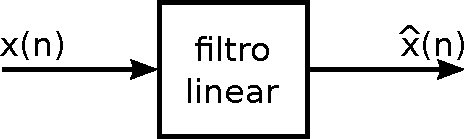
\includegraphics[width=0.35\textwidth]{images/filtro_preditor_linear.pdf}
    \caption{Preditor Linear - filtro digital.}
    \label{fig:fpl}
  \end{figure}
\end{frame}


\subsection{Padrões para Codificação de Voz}
\begin{frame}[allowframebreaks]
  \frametitle{Padrões do ITU-T}
  G.7xx: Audio (Voz) Protocolos de Compressão (CODEC)
  \begin{description}
  \item[G.711] - Modulação por código de pulso (\emph{Pulse code modulation}, PCM) de frequências de voz em um canal de 64 kbps.
  \item[G.721] - Codificação por código de pulso adaptativo (ADPCM) a 32 kbit/s.
  \item[G.722] - Codificação de áudio 7 kHz a 64 kbit/s.
  \item[G.722.1] - Codificação a 24 e 32 kbit/s para operação de sistemas com mãos livres com baixa perda de quadros.
  \item[G.722.2] - Codificação de banda larga de voz a aproximadamente 16 kbit/s utilizando codificação de banda larga com múltiplas taxas adaptativa (\emph{adaptive muti-rate wideband}, AMR-WB).
  \item[G.726] - Codificação por código de pulso adaptativa a 40, 32, 24, 16 kbit/s (ADPCM).
  \item[G.727] - Codificação por código de pulso adaptativa a 5-, 4-, 3- e 2-bit/amostra.
  \item[G.728] - Codificação de voz a 16 kbit/s utilizando código de excitação com predição linear com baixo atraso.
  \item[G.729] - Codificação de voz a 8 kbit/s utilizando estrutura conjugada codificação com excitação por códio algébrico e predição linear (\emph{conjugate-structure algebraic-code-excited linear-prediction}, CS-ACELP).
  \end{description}
\end{frame}


\begin{frame}
  \frametitle{Codificação de Voz}
  O sinal de fala é um sinal de áudio e é amostrado como qualquer outro sinal de áudio, mas
  devido à sua natureza particular (sinal de fala), ele possui propriedades que podem ser
  exploradas para obtermos uma compressão mais eficiente para este tipo de sinal.
\end{frame}


\begin{frame}
  \frametitle{Sinal de Voz}
  \begin{figure}[h]
  \centering
  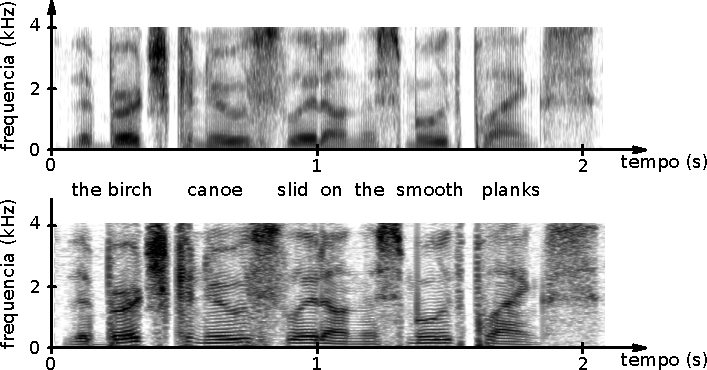
\includegraphics[width=0.85\textwidth]{images/spectrogram_birch_canoe.pdf}
  \caption{Espectrograma de uma sentença (a) banda-larga (b) banda-estreita.}
  \label{fig:specgram}
  \end{figure}
\end{frame}


\begin{frame}
  \frametitle{Trato Vocal}
  \begin{figure}[h]
  \centering 
  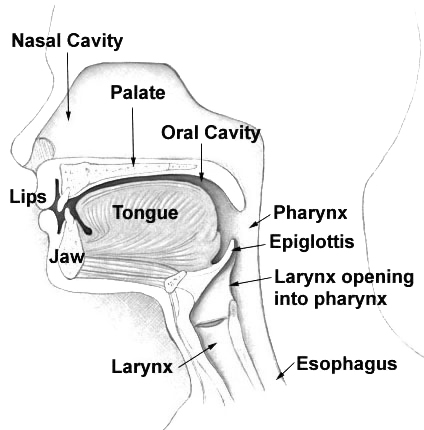
\includegraphics[width=0.4\textwidth]{images/head_neck.jpg}
  \caption{Aparato vocal humano (Wikipedia).}
  \label{fig:speech_apparatus}
  \end{figure}
\end{frame}


\begin{frame}
  \frametitle{Trato Vocal}
\begin{figure}
\centering
\begin{minipage}{.5\textwidth}
  \centering
  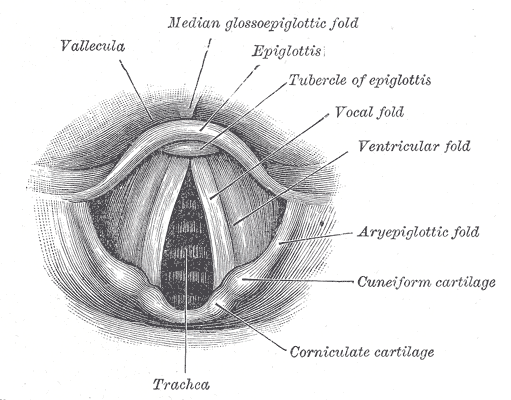
\includegraphics[width=.9\linewidth]{images/vocal_folds.png}
  \caption{Corte transversal \citep{gray1918}.}
  \label{fig:vocal_folds}
\end{minipage}%
\begin{minipage}{.5\textwidth}
  \centering
  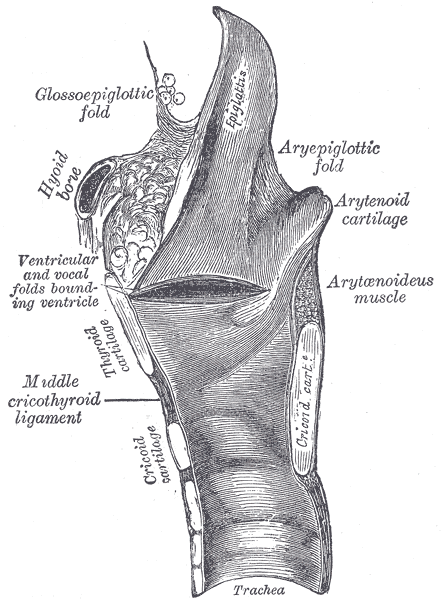
\includegraphics[width=.4\linewidth]{images/trachea.png}
  \caption{Corte sagital \citep{gray1918}.}
  \label{fig:trachea}
\end{minipage}
\end{figure}
\end{frame}

\begin{frame}
  \frametitle{Sinal de Voz}
  \begin{figure}[h]
  \centering  
  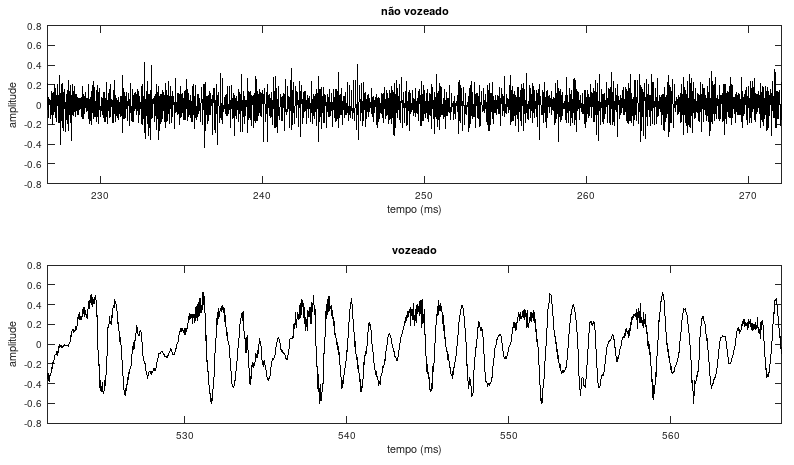
\includegraphics[width=0.7\textwidth]{images/vozeado.png}  
  \caption{(a) Vozeado e (b) Não-vozeado.}
  \label{fig:voice_unvoiced}  
  \end{figure}
\end{frame}

\begin{frame}
  \frametitle{Codificação de Voz}
  \begin{figure}[h]
  \centering
  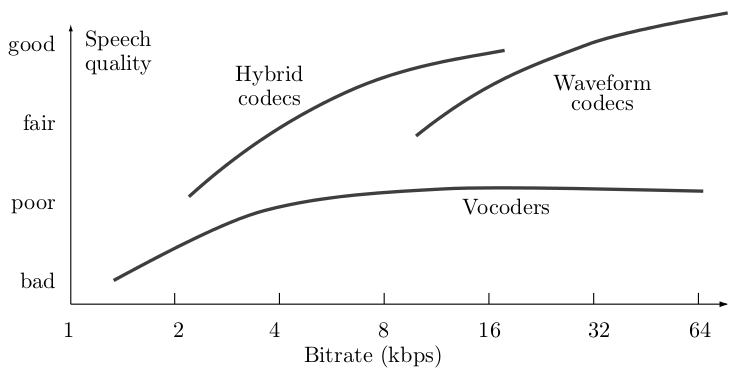
\includegraphics[width=0.7\textwidth]{images/speech_codecs.png}
  \caption{Qualidade da fala versus bitrate para abordagens distintas em codificações de voz.}
  \label{fig:speech_codecs}
  \end{figure}
\end{frame}

\begin{frame}
  \frametitle{Codificação de forma de onda}
  Este tipo de codificação não tenta predizer como o sinal original foi gerado.
  Apenas busca reproduzir, após a descompressão, as amostras de áudio que são
  o mais próximas possíveis das amostras originais.
  \begin{itemize}
  \item PCM
  \item ADPCM
  \item SBC (\emph{subband coding}) - codificação em sub-banda
  \item ATC (\emph{adaptive transform coding}) - codificação por transformação adaptativa
  \end{itemize}
\end{frame}

\begin{frame}
  \frametitle{ATC - codificação por transformação adaptativa}
   O arquivo de áudio é dividido em blocos de amostras e a DCT é aplicada
   em cada bloco, resultando em uma certa quantidade de coeficientes de frequências distintas.
   Cada coeficiente é quantizado de acordo com a sua frequência correspondente.
   É possível obter um sinal de áudio reconstruído com boa qualidade a taxas tão baixas quanto 16 kbps.
\end{frame}

\begin{frame}
  \frametitle{Codificação de Fonte}
  Um codificador de fonte utiliza um modelo matemático para a fonte produtora dos dados que desejamos codificar/transmitir.
  Se os dados originais correspondem a um sinal de voz, o codificador de fonte é chamado
  \emph{vocodes} (\emph{voice coder}). O exemplo mais comum é:
  \begin{itemize}
  \item LPC (linear predictive coder)
  \end{itemize}
\end{frame}


\subsection{LPC}
\begin{frame}
  \frametitle{LPC - linear predictive coding}
  \begin{figure}[h]
  \centering 
  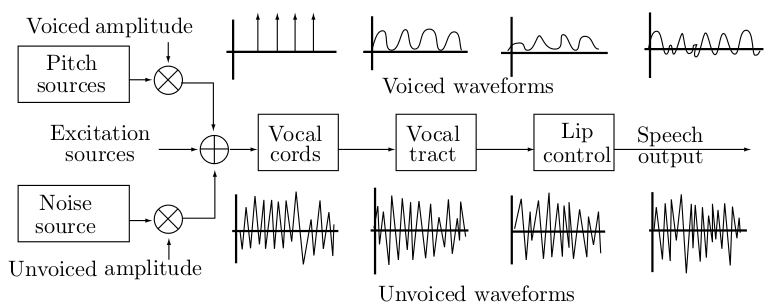
\includegraphics[width=0.75\textwidth]{/home/leoca/ee/ufsj/2012_01/audio_video/aulas/images/lpc_model.png}
  %\caption{.}
  \label{fig:lpc_model} 
  \end{figure}
\end{frame}


\begin{frame}
  \frametitle{LPC - codificação por predição linear}
  Utiliza-se um modelo de predição linear para representar o modelo do envelope de espectro de um trecho
  de um sinal de voz. Desta forma, não é necessário transmitir/armazenar as amostras do sinal de voz, mas apenas
  os parâmetros de excitação do filtro, o ganho e o filtro de predição linear.
  \begin{figure}[h]
  \centering 
  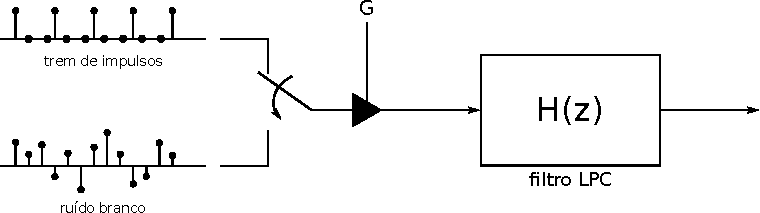
\includegraphics[width=0.75\textwidth]{images/lpc_scheme.pdf}
  %\caption{.}
  \label{fig:lpc} 
  \end{figure}
\end{frame}
\note{
\begin{scriptsize}
O LPC analisa o sinal de voz realizando um estimativa dos formantes, removendo o efeitos destes no sinal de fala,
e estimando a intensidade e frequência do zumbido remanescente. O processo de remover o efeito dos formantes
é chamado de filtragem inversa, e o sinal remanescente após a subtração do sinal modelado filtrado é chamado
de resíduo. Os parâmetros que descrevem a intensidade e frequência do zumbido, os formantes, e o sinal de resíduo,
podem ser armazenados ou transmitidos. A síntese LPC do sinal de fala utiliza o processo inverso:
utiliza os parâmetros do zumbido e o resíduo para criar sinal da fonte, utiliza os formantes para criar um filtro
(que representa a cavidade do trato vocal), e passa o sinal da fonte pelo filtro, resultando no sinal de fala.
Como o sinal de fala varia ao longo do tempo, este processo é feito em pequenos trechos de sinal de fala,
chamados quadros; usualmente de 30 a 50 quadros por segundo são utilizados para fornecer um sinal com boa
compressão e fala inteligível.
\end{scriptsize}
}
\note{
\begin{itemize}
\item LPC é usualmente utilizado para análise e ressíntese de sinal de voz.
\item Compressão de voz, como por exemplo no padrão GSM.
\item Transmissão sem fio, segura e encriptada de voz através um canal estreito; por exemplo: Navajo I, governo EUA.
\item Vocoders: aonde instrumentos musicais são utilizados como sinal de excitação para um filtro variante no tempo estimado a partir do sinal de voz de um cantor.
\item A predição feita pelo LPC é utilizada em codecs de áudio como por exemplo: Shorten, MPEG-4 ALS, FLAC, e outros.
\end{itemize}
}

\begin{frame}
  \frametitle{Codificação LPC}
  O LPC determina os coeficientes de um preditor linear através da minimização do erro de predição
  no sentido dos mínimos quadrados (uma das abordagens).
  Ele encontra os coeficientes de um preditor de ordem $p$ (filtro FIR)
  que prediz o valor atual de uma série temporal real $x$ a partir de amostras passadas.
  \begin{equation}
  \hat{x}[n] = -a_2 x[n-1] - a_3 x[n-2] - \cdots - a_{p+1} x[n-p]
  \end{equation}

  \begin{figure}[h]
  \centering 
  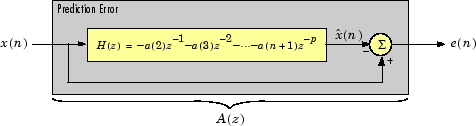
\includegraphics[width=0.65\textwidth]{images/reff2p100.png}
  \caption{Erro de predição. \url{https://www.mathworks.com/help/signal/ref/lpc.html} (Mathworks).}
  \label{fig:reff2p100} 
  \end{figure}

\end{frame}
\note{
  O erro de predição, $e[n]$, pode ser visto como a saída do filtro de predição $A(z)$, onde $H(z)$ é o preditor
  linear ótimo, $x[n]$ é o sinal de entrada, e $\hat{x}[n]$ é o sinal predito.

  \vspace{0.5cm}
  LPC utiliza o método da autocorrelação da modelagem auto-regressiva (AR) para encontrar os coeficientes de filtro.
  O filtro gerado pode não modelar o processo exatamente, mesmo que a sequência de dados seja efetivamente proveniente
  de um modelo AR com ordem correta $p$ adotada. Isto ocorre porque o método de autocorrelação implicitamente
  janela o sinal, isto é, assume que as amostras do sinal além do comprimento de $x$ sejam nulas.
}

\begin{frame}[allowframebreaks]
  \frametitle{Otimização baseada nos mínimos quadrados}
  O erro total é definido
  \begin{equation}
  \label{eq:err-total}
  \varepsilon = \sum_{n=n_0}^{n_1} e^2[n] ,
  \end{equation}
  aonde $n_0$ e $n_1$ compreendem o limite da extensão sobre a qual será realizada a otimização.
  Como temos
  \begin{equation}
  \label{eq:err-min-sqr-lpc}
  e[n] = x[n] - \hat{x}[n] = x[n] + \sum_{i=1}^p a_i x[n-i] = \sum_{i=0}^p a_i x[n-i] ,
  \end{equation}
  onde consideramos $a_0 = 1$.
  Substituindo \ref{eq:err-min-sqr-lpc} em \ref{eq:err-total} teremos:
  \begin{eqnarray}
  \varepsilon &=& \sum_{n=n_0}^{n_1} \left[ \sum_{i=0}^p a_i x[n-i] \right]^2 = \sum_{n=n_0}^{n_1} \sum_{i=0}^p \sum_{j=0}^p a_i x[n-i] x[n-j] a_j  \nonumber \\
              &=& \sum_{i=0}^p \sum_{j=0}^p a_i c_{ij} a_j ,
  \end{eqnarray}
  onde
  \begin{equation}
  c_{ij} = \sum_{n=n_0}^{n_1} x[n-i] x[n-j] .
  \end{equation}
  Para minimizar $\varepsilon$ em relação aos coeficientes do LPC, $a_1, a_2, \ldots, a_p$,
  devemos fazer a derivada parcial, em relação a cada coeficiente, igual a zero e resolver o sistema
  de equações remanescente.
  \begin{equation}
  \frac{\partial \varepsilon}{\partial a_k} = 2 \sum_{i=0}^p a_i c_{ik} = 0 .
  \end{equation}
  Como $a_0=1$, teremos então o sistema de equações normais:
  \begin{equation}
  \sum_{i=1}^p a_i c_{ik} = - c_{0k} , \quad k=1,2,\ldots,p .
  \end{equation}
  Obtemos assim um sistema linear $p\times p$ cuja solução é obtida diretamente pela inversão matricial
  (complexidade $O(p^3)$, mas existe forma mais eficiente para resolver este sistema).
\end{frame}

\begin{frame}[allowframebreaks]
  \frametitle{Método da Autocorrelação}
  O método da autocorrelação escolhe os limites $n_0=\infty$ e $n_1=\infty$, e ao mesmo tempo,
  força $x[n]=0$ para $n<0$ e $n\geq N$, i.e., limita o sinal a uma janela de tamanho $N$.
  Teremos então $c_{ij}$ dado pela função de autocorrelação $r(\tau)$:
  \begin{eqnarray}
  c_{ij} &=& \sum_{n=-\infty}^{\infty} x[n-i] x[n-j] \nonumber \\
         &=& \sum_{n=0}^{N-1-\vert i-j \vert} x[n] x[n+\vert i-k \vert] = r(\vert i-k \vert) .
  \end{eqnarray}
  Devido ao truncamento para zero de $x[n]$ fora de uma janela de $N$ amostras, teremos o equivalente
  à minimização do erro no intervalo $0 \leq n \leq N+p-1$.

  O sistema 
  \begin{equation}
  \sum_{i=1}^p a_i c_{ik} = - c_{0k} , \quad k=1,2,\ldots,p .
  \end{equation}
  será então reescrito como
  \begin{equation}
  \sum_{i=1}^p a_i r(\vert i-k \vert) = - r(k) , \quad k=1,2,\ldots,p .
  \end{equation}
  onde
  \begin{equation}
  r(\tau) = \sum_{n=0}^{N-1-\vert i-\tau}x[n] x[n+\tau] , \quad \tau \geq 0 .
  \end{equation}
  O erro de predição do sinal será
  \begin{equation}
  e[n] = x[n] + \sum_{i=1}^p a_i x[n-i] , \quad n=0,1,2,\ldots,N+p-1 .
  \end{equation}

  \framebreak
  Podemos também fazer a representação matricial do sistema de equações
  \begin{equation}
  \mathbf{X} \mathbf{a} = \mathbf{b}
  \end{equation}
  onde
  \begin{scriptsize}
  \begin{tabular}{ccc}
  $
  \mathbf{X} = 
  \left[ \begin{array}{cccc}
  x[0]   & 0      & \cdots & 0 \\
  x[1]   & x[0]   & \ddots & \vdots \\
  \vdots & x[1]   & \ddots & 0 \\
  x[N-1] & \vdots   & \ddots & x[0] \\
  0      & x[N-1]   & \ddots & x[1] \\
  \vdots & \ddots & \ddots & \vdots \\
  0      & \cdots &  0     & x[N-1]
  \end{array} \right] $,
  &
  $\mathbf{a} = \left[ \begin{array}{c}
  1 \\
  a[1] \\
  \vdots \\
  a[p] \end{array} \right] $

  &

  $\mathbf{b} = \left[ \begin{array}{c}
  x[0] \\
  0 \\
  \vdots \\
  0 \end{array} \right] $  .
  \end{tabular}
  \end{scriptsize}

  \framebreak
  Fazendo
  \begin{equation}
  \mathbf{X}^H \mathbf{X} \mathbf{a} = \mathbf{X}^H \mathbf{b}
  \end{equation}
  teremos as equações de Yule-Walker
  \begin{equation}
  \left[ \begin{array}{cccc}
  r[0]     & r[1]^\ast  & \cdots & r[p-1]^\ast \\
  r[1]     & r[0]       & \ddots & \vdots \\
  \vdots   & \ddots     & \ddots & r[1]^\ast  \\
  r[p-1]   & \cdots     & r[1]   & r[0] 
  \end{array} \right]
  \left[ \begin{array}{c} a[1] \\ a[2] \\ \vdots \\ a[p] \end{array} \right]
  =
  \left[ \begin{array}{c} -r[1] \\ -r[2] \\ \vdots \\ -r[p] \end{array} \right]
  \end{equation}
  que podem ser resolvidas pelo algoritmo de Levinson-Durbin com ordem de complexidade $O(p^2)$.

\end{frame}




\subsection{Codecs Híbridos}
\begin{frame}
  \frametitle{Codificação Híbrida}
  Os codecs híbridos combinam características de ambos: codificação de forma de onda e codificação de fonte.
  O mais popular dos codecs híbridos são os algorismos no domínio do tempo de `Análise através da Síntese',
  AbS (\emph{Analysis-by-Synthesis}).
\end{frame}


\begin{frame}
  \frametitle{Analysis-by-Synthesis (AbS)}
  Os codificadores AbS começam com um conjunto de amostras de fala (um quadro),
  codifica-as de forma similar ao LPC, decodifica, e subtrai o resultado da decodificação
  do sinal original. A diferença sofre um processo de minimização do erro que fornece
  amostras melhor codificadas. Estas amostras são novamente decodificadas, subtraídas das amostras
  originais, e novas diferenças são calculadas. Este processo é repetido até que as diferenças
  satisfaçam uma determinada condição para terminar o processo. O codificado procede então para
  o próximo quadro.
\end{frame}



\begin{frame}
  \frametitle{CELP - Code-excited linear prediction}
  Uma das codificações mais conhecidas do tipo AbS é o CELP, um acronismo que significa
  predição linear por excitação por código.
  \begin{itemize}
  \item Proposto em 1985 por M.R. Schroeder e B.S. Atal.
  \item É atualmente o algoritmo de codificação de voz mais utilizado.
  \item Utilizado no padrão para codificação de voz do MPEG-4 Audio.
  \end{itemize}
\end{frame}


\begin{frame}
  \frametitle{CELP - principais ideias}
  \begin{itemize}
  \item Utilizar o modelo fonte-filtro da produção da fala através da predição linear (LP).
  \item Utilizar um codebook adaptativo e fixo como entrada (excitação) do modelo LP.
  \item Buscar em um loop fechado em um domínio ponderado pelas características perceptivas.
  \item Quantização vetorial.
  \end{itemize}
\end{frame}


\begin{frame}
  \frametitle{Codificador CELP}
  \begin{figure}[h]
  \centering 
  \includegraphics[width=0.75\textwidth]{/home/leoca/ee/ufsj/2012_01/audio_video/aulas/images/celp.png}
  %\caption{.}
  \label{fig:celp}
  \end{figure}
\end{frame}


\begin{frame}
  \frametitle{Decodificador CELP}
  \begin{figure}[h]
  \centering 
  \includegraphics[width=0.5\textwidth]{/home/leoca/ee/ufsj/2012_01/audio_video/aulas/images/Celp_decoder.png}
  \caption{Decodificador CELP (Wikipedia).}
  \label{fig:Celp_decoder}
  \end{figure}
\end{frame}
\note{
A excitação é produzida pela soma das contribuições de um codebook adaptativo (aka pitch) e
um codebook estocástico (aka fixo). O codebook fixo é quandizado vetorialmente utilizando um
dicionário que é previamente definido no codec. As entradas do codebook adaptativo consistem
em versões atrasadas da excitação. Isto torna possível codificar eficientemente sinais periódicos,
tais como sinais vozeados. O filtro que molda a excitação é constituído por um modelo com
apenas pólos obtido através da predição linear.
}
\note{
A codificação (análise) é realizada através de uma otimização perceptiva do sinal decodificado (síntese)
em um loop fechado, utilizando uma função perceptiva simples de ponderação. A codificação é realizada
seguindo a seguinte ordem:
\begin{enumerate}
\item Os coeficientes LPC são calculados e quantizados.
\item É realizada uma busca no codebook adaptativo (pitch) e sua contribuição é removida.
\item É realizada a busca no codebook fixo.
\end{enumerate}
}

\begin{frame}%[allowframebreaks]
  \frametitle{Notebook - LPC vogais}
  \centering
  
\includegraphics[width=0.4\textwidth]{images/qrcode-jupyter-lpc-vowel.pdf}

  \url{https://nbviewer.jupyter.org/github/leolca/notebooks/blob/master/aev/lpc_vowels_formants.ipynb}
\end{frame} 

\begin{frame}%[allowframebreaks]
  \frametitle{Notebook - LPC síntese}
  \centering
  
\includegraphics[width=0.4\textwidth]{images/qrcode-jupyter-lpc-synthesis.pdf}

  \url{https://nbviewer.jupyter.org/github/leolca/notebooks/blob/master/aev/lpc-synthesis.ipynb}
\end{frame} 


\begin{frame}
  \frametitle{Leitura}
  Sugestão de leitura:
  \begin{itemize}
  \item \bibentry{Makhoul1975}
  \item \bibentry{salomon2010}
  \item \bibentry{kondoz2004} 
  \end{itemize}
\end{frame} 


